\section{Data}
\section{Snell's Law}
\subsection{Air to Glass}

\subsection{Glass to Air}

\begin{figure}[h]
    \centering
    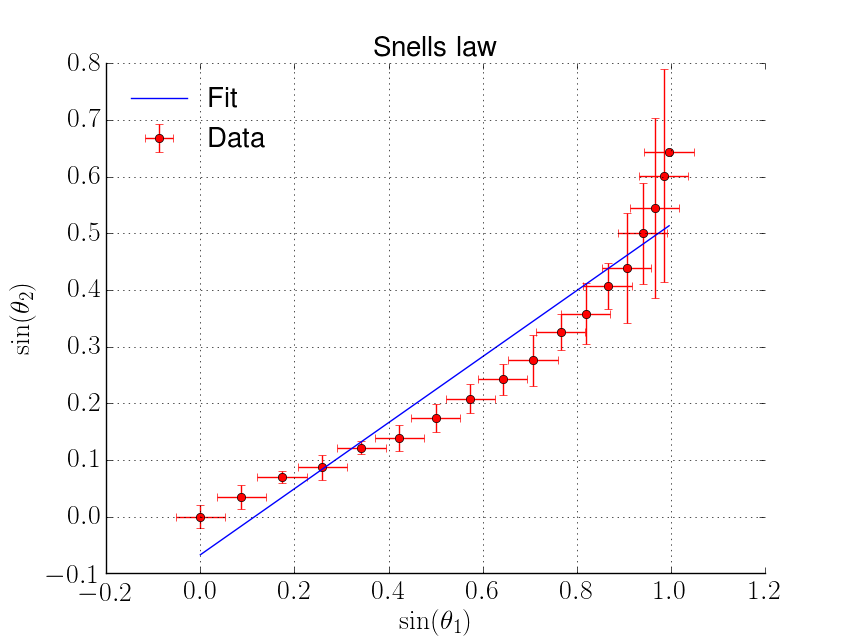
\includegraphics[width=0.5\textwidth]{snell}
    \caption{Dat\ldots}
    \label{fig:fit}
\end{figure}

\section{Reflection}
\subsection{p-polarized}
\subsection{s-polarized}
\begin{figure}[h]
    \centering
    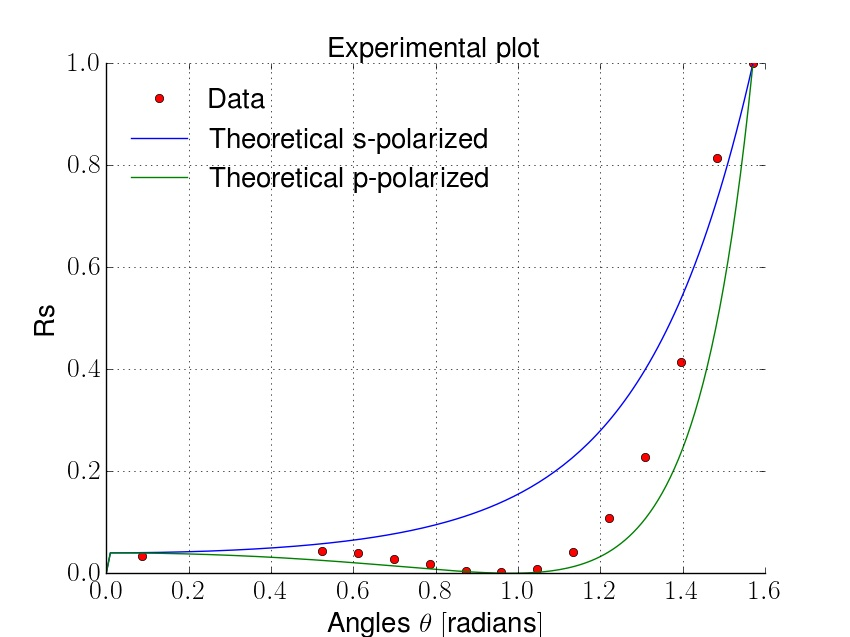
\includegraphics[width=0.5\textwidth]{reflection}
    \caption{Dat\ldots}
    \label{fig:reflection}
\end{figure}



\section{Transmission}
\subsection{p-polarized}
\subsection{s-polarized}
\begin{figure}[h]
    \centering
    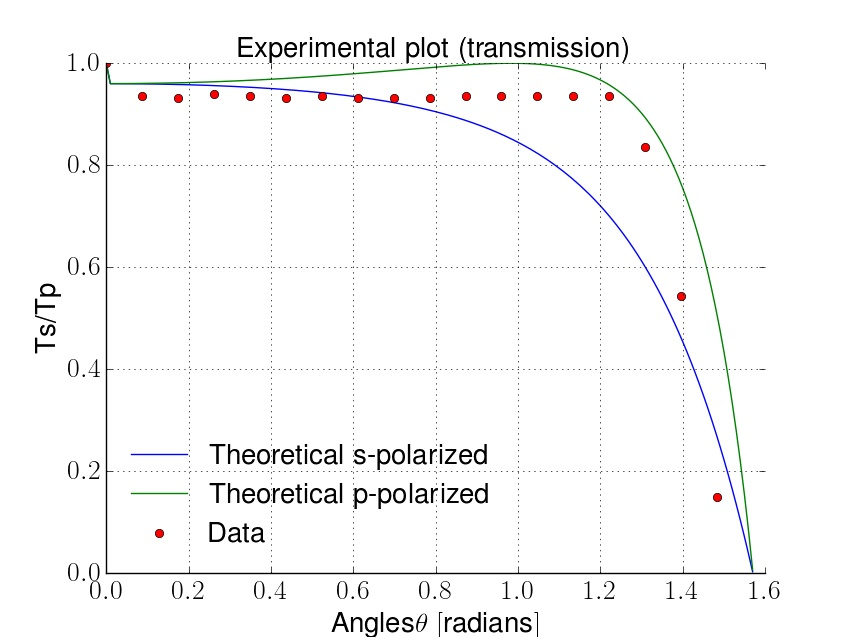
\includegraphics[width=0.5\textwidth]{transmission}
    \caption{Dat\ldots}
    \label{fig:transmission}
\end{figure}


